% !TEX encoding = UTF-8
% !TEX TS-program = pdflatex
% !TEX root = ../tesi.tex

%**************************************************************
\chapter{Analisi e progettazione}
\label{cap:analisi}
%**************************************************************

\intro{Il seguente capitolo descrive l'analisi, la progettazione iniziale, e le soluzioni addottate durante la codifica}\\


%**************************************************************
\section{Analisi e progettazione iniziale}
Le funzionalità da implementare e gli obbiettivi da raggiungere erano già ben definiti all'inizio del progetto, in quanto l'analisi funzionale è stata fornita dal \textit{product owner} insieme a una prima definizione del \textit{product backlog}.
Per questo motivo la fase di analisi dei requisiti da parte del \textit{team} di sviluppo è stata molto breve e si è concentrata principalmente su come le funzionalità del prodotto dovessero essere fruibili all'utente finale. La progettazione del \textit{software} non è avvenuta solamente all'inizio, ma si è protratta durante tutto il periodo di stage. Questo ha garantito maggior flessibilità nell'implementazione delle funzionalità e ha favorito l'utilizzo di Scrum. Tale scelta tuttavia ha anche introdotto il rischio che una debole progettazzione iniziale potesse causare problemi nelle settimane a venire. Questo rischio è stato subito mitigato grazie ad un attenta progettazione della base di dati pensando, nel miglior modo possibile, alle entità, a come esse fossero in relazione tra di loro e alla logica necessaria per implementare le funzionalità richieste. Inoltre, in quanto \textit{JHipster} utilizza uno \textit{stack} tecnologico ben definito, e impone dei vincoli architetturali da seguire, tale rischio è ulteriormente ridotto poiché non è necessario progettare l'architettura del \textit{software}.
Nel corso di questo capitolo vengono descritte le principali attività di progettazione svolte durante il corso dello stage.

%**************************************************************
\section{Progettazione del database}
La progettazione del \textit{database} è stata una delle attività più importanti, deteneva infatti un alto grado di priorità anche nel \textit{product backlog}. La progettazione del \textit{database} è stata divisa in due parti: la prima mirata a individuare le entità partendo dall'analisi dei requisiti fatta dal \textit{product owner}, mentre la seconda mettendo in relazione tali entità e aggiungendo tabelle se necessario. Per quanto riguarda la vera e propria implementazione del \textit{database} è stato sfruttato un tool fornito da \textit{JHipster} ovvero \href{https://start.JHipster.tech/jdl-studio/}{JDL-Studio}, che verrà descritto in modo dettagliato successivamente nel corso di questa sezione.

\subsection{Entità}
Durante la progettazione della base di dati sono state definite le entità descritte di seguito.
Per ciascuna di esse viene riportata una breve descrizione e la lista dei campi dati corredata dal tipo di dato. Nella lista seguente non vengono riportate chiavi primarie ne chiavi esterne poiché l'inserimento di tali campi dati è automatizzato e verrà descritto dettagliatamente nella sezione relativa alle \hyperref[rel]{relazioni tra entità}.
Mentre si stava effettuando la progettazione del \textit{database} è sorto il problema di come si volessero salvare i \gls{contenutog} e i \textit{template}. Si è optato di suddividere i contenuti in pagine, ognuna delle quali può contenere uno o più elementi multimediali e/o testuali. Inoltre in uno stesso contenuto si può selezionare un \textit{template} diverso per ogni pagina. Per quanto riguarda i \textit{template}, i quali sono definiti a monte dal \textit{team} di sviluppo, si è scelto di strutturarli definendo un \textit{template} al cui interno sono contenuti vari item che possono essere sia testuali che multimediali. Questo rende tutto il più modulare possibile, in quanto non pone limiti né in fase di creazione di un contenuto, né nella definizione dei \textit{template} e nel loro utilizzo. 
\subsubsection{Content}
Definisce un contenuto informativo, i suoi campi dati sono:
\begin{itemize}
    \item \textit{name (String)}: Nome del contenuto;
    \item \textit{state (State)}: Enumerazione che definisce i possibili stati di un contenuto;
    \item \textit{description (String)}: descrizione del contenuto informativo;
    \item \textit{slideTime (Integer)}: durata delle slide di un contenuto;
\end{itemize}

\subsubsection{ContentPage}
Definisce una pagina inserita in un contenuto. Ogni contenuto può avere più pagine che scorrono come slide durante la visualizzazione dello stesso; ogni pagina contiene degli item multimediali o testuali. I suoi campi dati sono:
\begin{itemize}
    \item \textit{pageNumber (Integer)}: numero della pagina all’interno di un contenuto.
\end{itemize}

\subsubsection{MultimediaItem}
Definisce un item multimediale (immagine o video) contenuto in una pagina. I suoi campi dati sono:
\begin{itemize}
    \item \textit{path (String)}: percorso del file multimediale caricato sul server, nel caso il caricamento delle immagini avvenga su NAS;
    \item \textit{resolution (Resolution)}: enumerazione che definisce la risoluzione dell'immagine caricata;
    \item \textit{multimediaFile (Blob)}: file multimediale caricato su \textit{database}, nel caso il caricamento non avvenga su NAS;
\end{itemize}

\subsubsection{TextItem}
Definisce un testo contenuto in una pagina. I suoi campi dati sono:
\begin{itemize}
    \item \textit{text (Blob)}: contenuto testuale inserito in una pagina.
\end{itemize}

\subsubsection{Template}
Definisce un \textit{template} che utilizzabile dalle pagine di un contenuto. Ogni pagina può utilizzare \textit{template} definiti a monte che determinano come immagini, video e contenuti testuali vengono disposti nella pagina al momento della presentazione. I suoi campi dati sono:
\begin{itemize}
    \item \textit{previewImage (Blob)}: immagine di preview del \textit{template}, utilizzata per aiutare l'utente a capire come questo è definito;
    \begin{figure}[h]
        \begin{center}
        
\includegraphics[width=0.18\textwidth]{textImage50_50}
        \caption{Immagine di preview di un \textit{template} contenente un testo e un'immagine}
        \label{fig:figure15}
        \end{center}
    \end{figure}
    \item \textit{templateHTML (Blob)}: contiene l'html del \textit{template};
    \item \textit{name (String)}: Nome del \textit{template}.
\end{itemize}

\subsubsection{TemplateItem}
Definisce un \textit{item} all'interno di un \textit{template}. Per \textit{item} si intende un singolo testo, immagine o video. Questa entità viene utilizzata in fase di creazione e di visualizzazione di un contenuto ed è utilizzata per sapere cosa va inserito in una pagina che utilizza un determinato \textit{template}. 
I suoi campi dati sono:
\begin{itemize}
    \item \textit{description (String)}: descrizione dell'item del \textit{template} (e.g. video a schermo intero);
    \item \textit{type (itemType)}: enumerazione che definisce il contenuto che viene inserito in quell’area del \textit{template};
    \item \textit{templateArea (Integer)}: area del \textit{template} in cui un certo oggetto va inserito, utilizzato in fase di preview per inserire immagini, video e testi al posto giusto all'interno del \textit{template}.
\end{itemize}

\subsubsection{CSS}
Definisce il CSS utilizzato da uno o più \textit{template}. I suoi campi dati sono:
\begin{itemize}
    \item \textit{templateCSS (Blob)}: contiene il CSS utilizzato da uno o più \textit{template}.
\end{itemize}

\subsubsection{CustomAudit}
Entità definita per implementare il sistema di Audit. I suoi campi dati sono:
\begin{itemize}
    \item \textit{action (Action)}: enumerazione che definisce il tipo di azione registrata negli audit;
    \item \textit{description (String)}: descrizione dettagliata dell'azione effettuata;
    \item \textit{timestamp (Instant)}: data e ora in cui l'azione registrata è stata eseguita.
\end{itemize}

\subsubsection{User}
Entità predefinita in \textit{JHipster} contenente tutte le informazioni necessarie per registrare un utente. Per utilizzarla è sufficiente definire relazioni ad essa.

\subsection{Enumerazioni}
Durante la progettazione della base di dati, in alcuni casi, si è ritenuto necessario definire alcuni campi dati come enumerazione al posto di utilizzare una semplice stringa di testo.
Questo garantisce maggior controllo e impone vincoli che evitano il verificarsi di errori relativi all'utilizzo di nomi diversi per esprimere lo stesso concetto. Le enumerazioni definite durante la progettazione del \textit{database} sono le seguenti.

\subsubsection{State}
Lista dei possibili stati di un contenuto informativo, ovvero: \textit{CREATED, TO\textunderscore{}ASSOCIATE, ASSOCIATED, TO\textunderscore{}AUTHORIZE, AUTHORIZED, PUBLISHED}.

\subsubsection{Resolution}
Lista delle possibili risoluzioni di un elemento multimediale, ovvero: \textit{HIGH, MEDIUM, LOW}.

\subsubsection{ItemType}
Lista delle diverse tipologie di \textit{template} item, ovvero: \textit{IMAGE, VIDEO, TEXT}.

\subsubsection{Action}
Lista delle azioni da registrare nel sistema di auditing che possono essere effettuate da un utente, ovvero: \textit{CREATE, DELETE, UPDATE, AUTHENTICATION\textunderscore{}SUCCESS, AUTHENTICATION\textunderscore{}FAILURE, LOGOUT, TIMEOUT}.

\subsection{Relazioni}
\label{rel}
Di seguito vengono evidenziate le relazioni tra le entità descritte in precedenza e ne viene data una breve descrizione.
\subsubsection{Content-ContentPage}
Ogni \textit{Content} può avere una o più \textit{ContentPage}, ogni \textit{ContentPage} è inserita in un solo contenuto.
\subsubsection{Template-ContentPage}
Ogni \textit{template} può essere utilizzato da una o più \textit{ContentPage}, ogni \textit{ContentPage} utilizza un solo \textit{template}.
\subsubsection{ContentPage-MultimediaItem}
Ogni \textit{ContentPage} può contenere uno o più \textit{MultimediaItem}, ogni \textit{MultimediaItem} è contenuto in una sola pagina.
\subsubsection{ContentPage-TextItem}
Ogni \textit{ContentPage} può contenere uno o più \textit{TextItem}, ogni \textit{TextItem} è contenuto in una sola pagina.
\subsubsection{Template-TemplateItem}
Ogni \textit{template} ha al suo interno uno o più \textit{templateItem}, ogni \textit{templateItem} fa riferimento a un solo \textit{template}.
\subsubsection{MultimediaItem-TemplateItem}
Ogni \textit{MultimediaItem} può riferirsi ad un solo \textit{templateItem}, ad ogni \textit{templateItem} possono essere riferiti uno o più \textit{MultimediaItem}.
\subsubsection{TextItem-TemplateItem}
Ogni \textit{TextItem} può riferirsi ad un solo \textit{templateItem}, ad ogni \textit{templateItem} possono essere riferiti uno o più \textit{TextItem}.
\subsubsection{Content-User}
Ogni \textit{Content} è creato da un solo \textit{User}, ogni \textit{User} può creare uno o più \textit{content}.
\subsubsection{CSS-template}
Ogni \textit{template} può avere uno o più \textit{CSS}, ogni \textit{CSS} può essere utilizzato da uno o più \textit{template}.
\subsubsection{CustomAudit-User}
Ogni \textit{Audit} si riferisce ad un solo \textit{User}, ad ogni \textit{User} possono essere registrati uno o più \textit{Audit}.


\subsection{Implementazione}
\subsubsection{JDL-Studio}
\textit{JDL-Studio} è un \textit{tool} fornito da \textit{JHipster} che permette di definire lo schema entità-relazioni di un \textit{database} tramite un apposito linguaggio di \textit{scripting} chiamato, appunto, \textit{JDL}. Una delle funzionalità più utili di \textit{JDL-Studio} è la possibilità di visualizzare il modello ER, che viene automaticamente aggiornato a ogni modifica.
\newpage
\subsubsection{Definizione di un'entità in JDL-Studio}
Un'entità viene definita in \textit{JD}L specificando il suo nome e i suoi campi dati. Un esempio di definizione di un'entità è il seguente:
\begin{lstlisting}[caption={Definizione entità Content},label={lst:ent}]
entity Content {
  name String unique,
  state State,
  description String,
  slideTime Integer
}
\end{lstlisting}
\subsubsection{Definizione di un'enumerazione in JDL-Studio}
Un'enumerazione viene definita in \textit{JDL} specificandone il nome e i suoi possibili valori dati. Un esempio di definizione di un'entità è il seguente:
\begin{lstlisting}[caption={Definizione enumerazione State},label={lst:en}]
enum State {
  CREATED,
  TO_ASSOCIATE,
  ASSOCIATED,
  TO_AUTHORIZE,
  AUTHORIZED,
  PUBLISHED
}
\end{lstlisting}
\subsubsection{Definizione di una relazione in JDL-Studio}
Per definire una relazione in \textit{JDL} bisogna innanzitutto specificare il tipo di relazione (uno a uno, uno a molti, molti a molti). Fatto questo è sufficiente specificare l'entità di partenza della relazione e quella di arrivo. Un esempio di definizione di relazioni in \textit{JDL} è il seguente:
\begin{lstlisting}[caption={Definizione relazioni uno a molti},label={lst:rel}]
    relationship OneToMany {
        Content{page} to ContentPage{content},
        Template{page} to ContentPage{template},
        ContentPage{multimediaItem} to MultimediaItem{page},
        TemplateItem{multimediaItem} to MultimediaItem{templateItem},
        Template{templateItem} to TemplateItem{template},
        ContentPage{textItem} to TextItem{page},
        TemplateItem{textItem} to TextItem{templateItem}
      }
\end{lstlisting}
\newpage
\subsubsection{Modello ER}
Il modello ER autogenerato presenta imperfezioni nella visualizzazione delle relazioni, nonostante ciò e stato ritenuto sufficiente per gli scopi del progetto.
\begin{figure}[h]
    \begin{center}
    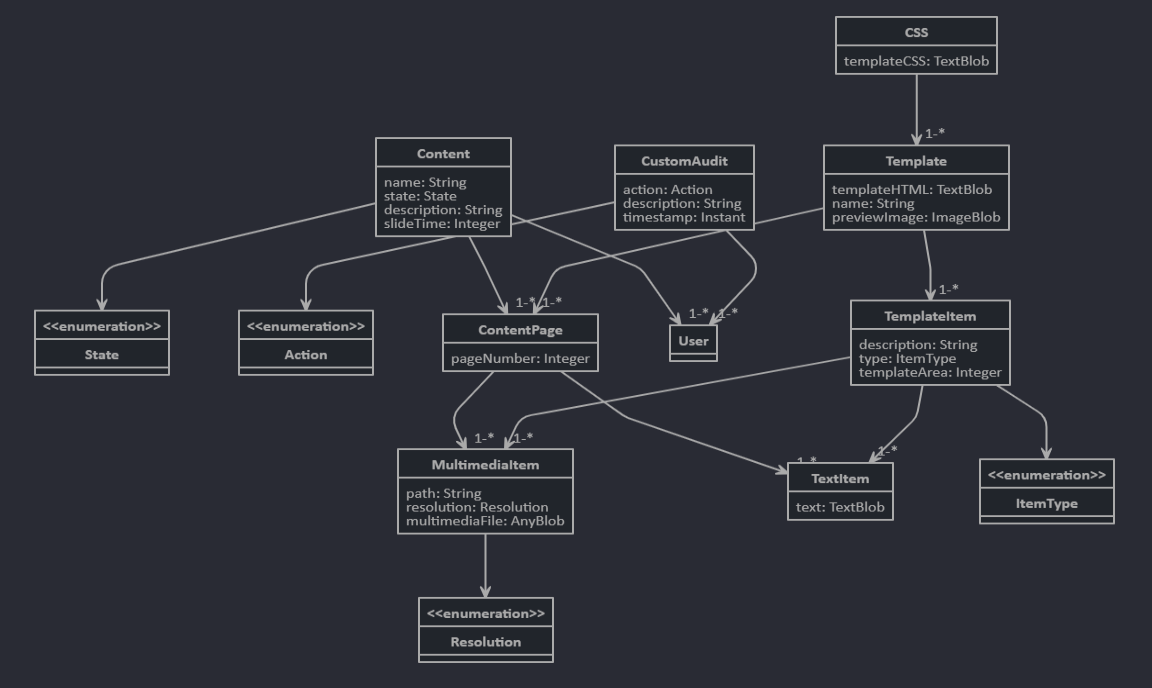
\includegraphics[width=1.2\textwidth]{er}
    \caption{Modello ER generato da JDL-Studio}
    \label{fig:figure19}
    \end{center}
\end{figure}
\\Una volta creato il modello del \textit{database} tramite \textit{JDL-Studio} è possibile importarlo direttamente all'interno dell'applicativo.
Tale procedura oltre a generare il \textit{database} crea anche una struttura di base dell'applicazione completa di \textit{back-end} e \textit{front-end}. Seppur questa non risulta completa di tutte le funzionalità necessarie, evita la scrittura di numerose linee di codice al programmatore riducendo l'introduzione di errori umani.
%**************************************************************
\section{Definizione dei template per i contenuti}
In quanto nella progettazione del \textit{database} è stato scelto di modellare i \textit{template} in modo che fossero più modulari ed estendibili possibile, è stata necessaria un'accurata definizione degli stessi. Si è optato per definire un \textit{template} di base utilizzato da ciascun contenuto informativo, e una serie di \textit{template} personalizzati utilizzati dalle pagine inserite in un contenuto.
\subsection{Template di base}
Il \textit{template} di base definito contiene poche informazioni. Definisce infatti la struttura base della pagina \textit{html} e la funzione per visualizzare le \textit{slide}. Contiene inoltre vari \textit{placeholder} utilizzati per inserire dinamicamente le informazioni di un determinato contenuto informativo.
I placeholder definiti sono: 
\begin{itemize}
    \item \textit{\$\{CSS\}}: Utilizzato per inserire il \textit{CSS} dei \textit{template} utilizzati;
    \item \textit{\$\{CONTENTID\}}: Utilizzato per inserire l’identificativo del contenuto come campo \textit{id} nel codice \textit{html};
    \item \textit{\$\{PAGES\}}: Utilizzato per inserire le pagine presenti in un contenuto;
    \item \textit{\$\{SLIDETIME\}}: Utilizzato per impostare lo slidetime scelto in un contenuto;
\end{itemize}
\subsection{Template di pagina}
I \textit{template} di pagina sono quelli scelti dall'utente durantela creazione di un contenuto.
Anche in questo caso i \textit{template}, scritti in \textit{html}, avranno al loro interno opportuni \textit{placeholder} per inserire i dati al momento dell'utilizzo. Poiché non si può sapere a priori come saranno definiti i \textit{template} futuri sono state definite delle regole da seguire durante la creazione di un nuovo \textit{template}. La lista delle regole definite è la seguente:
\begin{itemize}
    \item definire un nome del \textit{template} univoco;
    \item anteporre il nome del \textit{template} ad ogni classe o \textit{id} utilizzati per il \textit{CSS};
    \item non definire \textit{CSS} per gli elementi \textit{html} (e.g. H1, div, p), definirlo solamente classi e \textit{id};
    \item definire un tag \textit{<div>...</div>} differente per ogni \textit{item} del \textit{template};
    \item nel caso si volessero inserire video o immagini all'interno di un nuovo \textit{template} seguire gli esempi forniti insieme alla documentazione;
    \item definire i placeholder per l'inserimento di video, immagini o elementi testuali nel formato \textit{\$\{ItemType\textit{template}Area\}};
\end{itemize}

%**************************************************************
\section{Definizione dei servizi di back-end}
Durante l'importazione del modello del \textit{database} \textit{JHipster} genera automaticamente alcuni servizi \textit{RESTful} per ciascuna entità. Più nello specifico:
\begin{itemize}
    \item creazione di un \textit{record};
    \item eliminazione di un \textit{record};
    \item modifica di un \textit{record};
    \item ricerca di un \textit{record} per \textit{ID};
    \item ricerca di tutti i \textit{record} presenti;
\end{itemize}
I servizi autogenerati tuttavia non erano sufficienti allo scopo del \textit{software}, alcuni di essi hanno avuto la necessità di essere modificati mentre per altre funzionalità ne sono stati implementati di nuovi. I servizi con la necessità di essere adattati erano, in genere, quelli di modifica. Questi sono stati ridefiniti in modo che gestissero le relazioni correttamente. Sono stati inoltre modificati i servizi di eliminazione, in modo che rispettassero i vincoli di integrità referenziale
I servizi definiti ad hoc sono invece i seguenti:
\begin{itemize}
    \item servizio di \textit{update} dello stato di un contenuto;
    \item servizio di creazione della \textit{preview} di un contenuto;
    \item servizio di \textit{upload} di un file multimediale;
    \item servizio di ricerca di un file multimediale per \textit{ID} e che ritorna il file in \textit{Base64};
\end{itemize}
